%---------------------------------------------------------------------------%
%-                                                                         -%
%-                           LaTeX Template                                -%
%-                                                                         -%
%---------------------------------------------------------------------------%
%- Copyright (C) Huangrui Mo <huangrui.mo@gmail.com>
%- This is free software: you can redistribute it and/or modify it
%- under the terms of the GNU General Public License as published by
%- the Free Software Foundation, either version 3 of the License, or
%- (at your option) any later version.
%---------------------------------------------------------------------------%
%->> Document class declaration
%---------------------------------------------------------------------------%
\documentclass[singlesided]{Style/ucasthesis}%
%- Multiple optional arguments:
%- [<singlesided|doublesided|printcopy>]% set one or two sided eprint or print
%- [draftversion]% show draft version information
%- [fontset=<fandol|...>]% specify font set to replace automatic detection
%- [scheme=plain]% thesis writing of international students
%- [standard options for ctex book class: draft|paper size|font size|...]%
%---------------------------------------------------------------------------%
%->> Document settings
%---------------------------------------------------------------------------%
\usepackage[authoryear,myhdr,list]{Style/artratex}% document settings
%- usage: \usepackage[option1,option2,...,optionN]{artratex}
%- Multiple optional arguments:
%- [bibtex|biber]% set bibliography processor and package
%- [<numbers|super|authoryear|alpha>]% set citation and reference style
%- <numbers>: textual: Jones [1]; parenthetical: [1]
%- <super>: textual: Jones superscript [1]; parenthetical: superscript [1]
%- <authoryear>: textual: Jones (1995); parenthetical: (Jones, 1995)
%- <alpha>: textual: not available; parenthetical: [Jon95]
%- [geometry]% reconfigure page layout via geometry package
%- [lscape]% provide landscape layout environment
%- [myhdr]% enable header and footer via fancyhdr package
%- [color]% provide color support via xcolor package
%- [background]% enable page background
%- [tikz]% provide complex diagrams via tikz package
%- [table]% provide complex tables via ctable package
%- [list]% provide enhanced list environments for algorithm and coding
%- [math]% enable some extra math packages
\usepackage{Style/artracom}% user defined commands

%%%%%%%%%%%%%%
\usepackage{fancyvrb}
\usepackage{hologo}

% \setlength{\hfuzz}{3pt}
% \ctexset{linestretch = 2\ccwd}
% \setlength{\bibitemsep}{3bp}
% \renewcommand*{\bibfont}{\zihao{5}\linespread{1.27}\selectfont}

\hypersetup{colorlinks = true, allcolors = blue}
\newcommand{\myemph}[1]{\emph{\textcolor{red}{#1}}}
\newcommand{\unemph}[1]{\textup{\textcolor{black}{#1}}}
\newcommand{\docversion}{v1.7.4}

\newcommand{\tightlist}{%
  \setlength{\itemsep}{0pt}\setlength{\parskip}{0pt}}
\usepackage{longtable,booktabs}
%<-huxtable dependencies
\usepackage{threeparttable}
\usepackage{tabularx}
\usepackage{graphicx,grffile}
\usepackage{wrapfig}
\usepackage{siunitx}
\usepackage{colortbl}
\usepackage{multirow}
\usepackage{hhline}
\usepackage{calc}
\usepackage{placeins}
\usepackage{pmboxdraw}
%
\usepackage{amssymb,amsmath}
%\usepackage{natbib}
%\bibliographystyle{apalike}
\newcommand{\VerbBar}{|}
\newcommand{\VERB}{\Verb[commandchars=\\\{\}]}
\DefineVerbatimEnvironment{Highlighting}{Verbatim}{commandchars=\\\{\}}
% Add ',fontsize=\small' for more characters per line
\usepackage{framed}
\definecolor{shadecolor}{RGB}{248,248,248}
\newenvironment{Shaded}{\begin{snugshade}}{\end{snugshade}}
\newcommand{\KeywordTok}[1]{\textcolor[rgb]{0.13,0.29,0.53}{\textbf{{#1}}}}
\newcommand{\DataTypeTok}[1]{\textcolor[rgb]{0.13,0.29,0.53}{{#1}}}
\newcommand{\DecValTok}[1]{\textcolor[rgb]{0.00,0.00,0.81}{{#1}}}
\newcommand{\BaseNTok}[1]{\textcolor[rgb]{0.00,0.00,0.81}{{#1}}}
\newcommand{\FloatTok}[1]{\textcolor[rgb]{0.00,0.00,0.81}{{#1}}}
\newcommand{\ConstantTok}[1]{\textcolor[rgb]{0.00,0.00,0.00}{{#1}}}
\newcommand{\CharTok}[1]{\textcolor[rgb]{0.31,0.60,0.02}{{#1}}}
\newcommand{\SpecialCharTok}[1]{\textcolor[rgb]{0.00,0.00,0.00}{{#1}}}
\newcommand{\StringTok}[1]{\textcolor[rgb]{0.31,0.60,0.02}{{#1}}}
\newcommand{\VerbatimStringTok}[1]{\textcolor[rgb]{0.31,0.60,0.02}{{#1}}}
\newcommand{\SpecialStringTok}[1]{\textcolor[rgb]{0.31,0.60,0.02}{{#1}}}
\newcommand{\ImportTok}[1]{{#1}}
\newcommand{\CommentTok}[1]{\textcolor[rgb]{0.56,0.35,0.01}{\textit{{#1}}}}
\newcommand{\DocumentationTok}[1]{\textcolor[rgb]{0.56,0.35,0.01}{\textbf{\textit{{#1}}}}}
\newcommand{\AnnotationTok}[1]{\textcolor[rgb]{0.56,0.35,0.01}{\textbf{\textit{{#1}}}}}
\newcommand{\CommentVarTok}[1]{\textcolor[rgb]{0.56,0.35,0.01}{\textbf{\textit{{#1}}}}}
\newcommand{\OtherTok}[1]{\textcolor[rgb]{0.56,0.35,0.01}{{#1}}}
\newcommand{\FunctionTok}[1]{\textcolor[rgb]{0.00,0.00,0.00}{{#1}}}
\newcommand{\VariableTok}[1]{\textcolor[rgb]{0.00,0.00,0.00}{{#1}}}
\newcommand{\ControlFlowTok}[1]{\textcolor[rgb]{0.13,0.29,0.53}{\textbf{{#1}}}}
\newcommand{\OperatorTok}[1]{\textcolor[rgb]{0.81,0.36,0.00}{\textbf{{#1}}}}
\newcommand{\BuiltInTok}[1]{{#1}}
\newcommand{\ExtensionTok}[1]{{#1}}
\newcommand{\PreprocessorTok}[1]{\textcolor[rgb]{0.56,0.35,0.01}{\textit{{#1}}}}
\newcommand{\AttributeTok}[1]{\textcolor[rgb]{0.77,0.63,0.00}{{#1}}}
\newcommand{\RegionMarkerTok}[1]{{#1}}
\newcommand{\InformationTok}[1]{\textcolor[rgb]{0.56,0.35,0.01}{\textbf{\textit{{#1}}}}}
\newcommand{\WarningTok}[1]{\textcolor[rgb]{0.56,0.35,0.01}{\textbf{\textit{{#1}}}}}
\newcommand{\AlertTok}[1]{\textcolor[rgb]{0.94,0.16,0.16}{{#1}}}
\newcommand{\ErrorTok}[1]{\textcolor[rgb]{0.64,0.00,0.00}{\textbf{{#1}}}}
\newcommand{\NormalTok}[1]{{#1}}
%%%%%%%%%%%%%%


%---------------------------------------------------------------------------%
%->> Document inclusion
%---------------------------------------------------------------------------%
%\includeonly{Tex/Chap_1,...,Tex/Chap_N}% selected files compilation
%---------------------------------------------------------------------------%
%->> Document content
%---------------------------------------------------------------------------%
\begin{document}
%-
%-> Frontmatter: title page, abstract, content list, symbol list, preface
%-
\frontmatter% initialize the environment

%---------------------------------------------------------------------------%
%->> 封面信息及生成
%---------------------------------------------------------------------------%
%-
%-> 中文封面信息
%-
\confidential{}% 密级:只有涉密论文才填写
\schoollogo{scale=0.5}{zuel_logo}% 校徽
\title{中南财经政法大学本科生学位论文 bookdown 模板(非官方)}% 论文中文题目
\author{donk3yzz}% 论文作者
\advisor{谷哥教授}% 指导教师:姓名 专业技术职务 工作单位
\advisorsec{}% 指导老师附加信息 或 第二指导老师信息
\degree{学士}% 学位:学士、硕士、博士
\degreetype{理学}% 学位类别:理学、工学、工程、医学等
\major{论文排版}% 二级学科专业名称
\institute{R 语言学院}% 院系名称
\chinesedate{2018 年 9 月}% 毕业日期:夏季为6月、冬季为12月
%-
%-> 英文封面信息
%-
\englishtitle{Zhongnan University of Economics and Law undergraduate graduation thesis template}% 论文英文题目
\englishauthor{Feng, Shengshi}% 论文作者
\englishadvisor{Supervisor: Prof.Google}% 指导教师
\englishdegree{Master}% 学位:Bachelor, Master, Doctor。封面格式将根据英文学位名称自动切换,请确保拼写准确无误
\englishdegreetype{Natural Science}% 学位类别:Philosophy, Natural Science, Engineering, Economics, Agriculture 等
\englishthesistype{thesis}% 论文类型: thesis, dissertation
\englishmajor{Typesetting}% 二级学科专业名称
\englishinstitute{College of R}% 院系名称
\englishdate{September, 2018}% 毕业日期:夏季为June、冬季为December
%-
%-> 生成封面
%-
\maketitle% 生成中文封面
%\makeenglishtitle% 生成英文封面
%-
%-> 作者声明
%-
%
%
\makedeclaration% 生成声明页
\makezueltitle% 生成中南财经政法大学论文标题面
%-
%-> 中文摘要
%-
\setcounter{page}{1}% 开始页码
\pagenumbering{arabic}% 页码符号
%\chapter{摘要}%\chaptermark{摘\quad要}% 摘要标题
%这里写中文摘要。啊不可挡家真的好。
%\keywords{排版;文档类}% 中文关键词

\cabstract{这里写中文摘要。啊不可挡家真的好。}{排版;文档类}
%-
%-> 英文摘要
%-
\chapter*{Abstract}%\chaptermark{Abstract}% 摘要标题
%

\englishkeywords{\hologo{LaTeX2e}, \CTeX{}, bookdown}% 英文关键词
%
%---------------------------------------------------------------------------%



{% content list region
\linespread{1.2}% local line space
%\intotoc{\contentsname}% add link to contents table and bookmark
\tableofcontents% contents catalog
%\intotoc{\listfigurename}% add link to contents table and bookmark
\listoffigures% figures catalog
%\intotoc{\listtablename}% add link to contents table and bookmark
\listoftables% tables catalog
}
\chapter*{符号列表}
\chaptermark{符号列表}

\section*{字符}
\nomenclatureitem[\textbf{Unit}]{\textbf{Symbol}}{\textbf{Description}}
\nomenclatureitem[$\Unit{m^{2} \cdot s^{-2} \cdot K^{-1}}$]{$R$}{the gas constant}
\nomenclatureitem[$\Unit{m^{2} \cdot s^{-2} \cdot K^{-1}}$]{$C_v$}{specific heat capacity at constant volume}
\nomenclatureitem[$\Unit{m^{2} \cdot s^{-2} \cdot K^{-1}}$]{$C_p$}{specific heat capacity at constant pressure}
\nomenclatureitem[$\Unit{m^{2} \cdot s^{-2}}$]{$E$}{specific total energy}
\nomenclatureitem[$\Unit{m^{2} \cdot s^{-2}}$]{$e$}{specific internal energy}
\nomenclatureitem[$\Unit{m^{2} \cdot s^{-2}}$]{$h_T$}{specific total enthalpy}
\nomenclatureitem[$\Unit{m^{2} \cdot s^{-2}}$]{$h$}{specific enthalpy}
\nomenclatureitem[$\Unit{kg \cdot m \cdot s^{-3} \cdot K^{-1}}$]{$k$}{thermal conductivity}
\nomenclatureitem[$\Unit{kg \cdot m^{-1} \cdot s^{-2}}$]{$S_{ij}$}{deviatoric stress tensor}
\nomenclatureitem[$\Unit{kg \cdot m^{-1} \cdot s^{-2}}$]{$\tau_{ij}$}{viscous stress tensor}
\nomenclatureitem[$\Unit{1}$]{$\delta_{ij}$}{Kronecker tensor}
\nomenclatureitem[$\Unit{1}$]{$I_{ij}$}{identity tensor}

\section*{算子}
\nomenclatureitem{\textbf{Symbol}}{\textbf{Description}}
\nomenclatureitem{$\Delta$}{difference}
\nomenclatureitem{$\nabla$}{gradient operator}
\nomenclatureitem{$\delta^{\pm}$}{upwind-biased interpolation scheme}

\section*{缩写}
\nomenclatureitem{CFD}{Computational Fluid Dynamics}
\nomenclatureitem{CFL}{Courant-Friedrichs-Lewy}
\nomenclatureitem{EOS}{Equation of State}
\nomenclatureitem{JWL}{Jones-Wilkins-Lee}
\nomenclatureitem{WENO}{Weighted Essentially Non-oscillatory}
\nomenclatureitem{ZND}{Zel'dovich-von Neumann-Doering}

% list of symbols, preface content
%-
%-> Mainmatter
%-

\setcounter{page}{1}
\mainmatter% initialize the environment
\mainmatter

\hypertarget{introduction}{%
\chapter{引言}\label{introduction}}

作为一个懒人,本人比较喜欢用一些工作减少自己的重复性劳动的时间,然鹅往往为了这些东西消耗了更多时间,本篇就是这么个例子。

这是一个基于\texttt{bookdownplus-ucas\_zh}修改来的zuel毕业论文模版,已经基本上定制好了我财毕业论文的基本要求,所以在使用时可以体会markdown标记符号的简洁性,\texttt{knitr}输出R代码结果和包中的一些其他的函数,LaTex数学公式和交叉引用\ldots{}\ldots{}使用者可以在掌握一些LaTex排版知识后专心于论文写作。

除此之外,使用本模板的同时推荐使用\texttt{tinytex},它是一个基于TexLive改造的、非常节省系统空间的LaTex发行版,对于R用户,它可以对在knit过程中用到却没有的安装LaTex包自动下载,十分方便。

同时,bookdown包的输出方式除了pdf之外,还包括word、html、Gitbook等常见格式。除了论文与书籍的写作之外,你也可以在\texttt{bookdown-demo}或\texttt{bookdownplus}中寻找一些明信片之类的模板。

应该值得注意的是,本模板是在\texttt{bookdownplus-ucas\_zh}基础上调参和略微修改之后的结果,你可以在项目内看到各种属于原模板的痕迹,同时由于本人也没有系统学习过LaTex知识,代码规范方面也是心有余而力不足,所以本模板除了方便的输出ZUEL毕业论文以外没有任何参考价值。如果在使用中遇到问题,欢迎在GitHub issue中提出。

\hypertarget{acknowlage}{%
\chapter{致谢}\label{acknowlage}}

首先要感谢yihui,毕竟创世神;还有zhao peng,他改造了ucas毕业论文的LaTex模板使之适用于bookdown,并在我准备对模板继续改造时提供了非常关键的帮助。

追本溯源的话,应该还有pandoc,甚至Ctex的开发者,就不多言了。

\hypertarget{start}{%
\chapter{开始使用}\label{start}}

\hypertarget{section}{%
\section{使用环境}\label{section}}

为了保证你在使用本模板时有一个愉快的体验,你的电脑应该配置有:

\begin{itemize}
\tightlist
\item
  3.5.0版本以上的R
\item
  最新版本的Rstudio
\item
  2.7版本以上的pandoc
\item
  最新版本的TinyTex(推荐,相关内容可以参考\_\_\_\_待补充 )
\end{itemize}

\hypertarget{first-use}{%
\section{第一次使用}\label{first-use}}

在配置好上面的环境之后,你可以在\href{https://github.com/donk3yzz/zuel_zh}{donk3yzz/zuel\_zh}下载本模板,然后打开模板的\texttt{bookdown-plus.rproj},点击Rstudio中的\texttt{build\ book}或按快捷键\texttt{ctrl+shift+b},文档会开始编译并且下载需要的Tex包,这一过程通常要持续几分钟,下载并编译完成后\texttt{\_book/zuel\_zh.pdf}即论文模板的成稿。

\hypertarget{bookdown}{%
\chapter{bookdown组件}\label{bookdown}}

本章内容包括在使用模板撰写论文时常用的bookdown组件,包括代码块、图片、表格、引用、数学定理与方程。本章的大部分内容翻译自https://bookdown.org/yihui/bookdown/components.html。由于bookdown的建立是基于pandoc的,我们从一些pandoc语法开始。

\hypertarget{markdown}{%
\section{markdown语法}\label{markdown}}

\hypertarget{section-1}{%
\subsection{行内样式}\label{section-1}}

你可以通过\texttt{\_斜体\_}或\texttt{*斜体*}来使用\emph{斜体};用\texttt{**粗体**}或\texttt{\_\_粗体\_\_}来使用\textbf{粗体}。两个\texttt{\textasciitilde{}}中间的文字会变为下标如\texttt{X\textasciitilde{}1\textasciitilde{},X\textasciitilde{}2\textasciitilde{},\$\textbackslash{}cdots\$,X\textasciitilde{}n\textasciitilde{}},会生成X\textsubscript{1},X\textsubscript{2},\(\cdots\),X\textsubscript{n};同样俩个\texttt{\^{}}间的文字会变为上标如\texttt{X\^{}2\^{}}会生成X\textsuperscript{2}。超链接将使用\texttt{{[}text{]}(link)}创建,如\texttt{{[}RStudio{]}(https://www.rstudio.com)}\href{https://www.rstudio.com}{RStudio}。可以使用\texttt{\^{}{[}{]}}添加脚注,如\texttt{\^{}{[}这是一个脚注{]}}\footnote{这是一个脚注}

\hypertarget{section-2}{%
\subsection{数学表达式}\label{section-2}}

你可以在一对\texttt{\$}中间插入行内LaTex数学表达式,例如\texttt{\$f(k)\ =\ \{n\ \textbackslash{}choose\ k\}\ p\^{}\{k\}\ (1-p)\^{}\{n-k\}\$}会输出\(f(k) = {n \choose k} p^{k} (1-p)^{n-k}\),或者在一对\texttt{\$\$}中插入行间数学表达式,例如\texttt{\$\$f(k)\ =\ \{n\ \textbackslash{}choose\ k\}\ p\^{}\{k\}\ (1-p)\^{}\{n-k\}\$\$} 会输出 \[f(k) = {n \choose k} p^{k} (1-p)^{n-k}\]。

同样,你还可以在一对\texttt{\$}或\texttt{\$\$}中间使用其他数学环境,比如

\begin{verbatim}
$$
\begin{array}{ccc}
x_{11} & x_{12} & x_{13}\\
x_{21} & x_{22} & x_{23}
\end{array}
$$
\end{verbatim}

\[
\begin{array}{ccc}
x_{11} & x_{12} & x_{13}\\
x_{21} & x_{22} & x_{23}
\end{array}
\]

你可以引用更多的数学环境如矩阵、行列式等等,详情可以参考latex中文简介

\hypertarget{bookdownmarkdown}{%
\section{bookdown支持的markdown拓展}\label{bookdownmarkdown}}

为了有效的给数学公式标数字且引用,你可以在公式的数学环境中加入标签\texttt{(\textbackslash{}\#eq:标签)},并引用他们,例如:

\begin{Shaded}
\begin{Highlighting}[]
\KeywordTok{\textbackslash{}begin}\NormalTok{\{}\ExtensionTok{equation}\NormalTok{\}}\SpecialStringTok{ }
\SpecialStringTok{  f}\SpecialCharTok{\textbackslash{}left}\SpecialStringTok{(k}\SpecialCharTok{\textbackslash{}right}\SpecialStringTok{) = }\SpecialCharTok{\textbackslash{}binom}\SpecialStringTok{\{n\}\{k\} p^k}\SpecialCharTok{\textbackslash{}left}\SpecialStringTok{(1-p}\SpecialCharTok{\textbackslash{}right}\SpecialStringTok{)^\{n-k\}}
\SpecialStringTok{  (}\SpecialCharTok{\textbackslash{}#}\SpecialStringTok{eq:binom)}
\KeywordTok{\textbackslash{}end}\NormalTok{\{}\ExtensionTok{equation}\NormalTok{\}}
\end{Highlighting}
\end{Shaded}

将得到:
\begin{equation} 
  f\left(k\right) = \binom{n}{k} p^k\left(1-p\right)^{n-k}
  \label{eq:binom}
\end{equation}

那么你就可以使用\texttt{\textbackslash{}@ref(eq:binom)}来引用此公式,例如见\eqref{eq:binom}

\hypertarget{theorems-proof}{%
\section{定理与证明}\label{theorems-proof}}

bookdown中支持另一种定理环境,是基于code chunk来完成的,例如

输出结果为:

在引用时你可以使用\texttt{\textbackslash{}@ref(prefix:label)},prefix是定理环境的简写,对于theorem为thm,那么我们要引用此定理,就可以用\texttt{\textbackslash{}@ref(thm:pyth)},即,见定理\ref{thm:pyth}

对于更多的定理环境以及他们对应的prefix可以见\href{https://bookdown.org/yihui/bookdown/markdown-extensions-by-bookdown.html\#theorems}{theorems}。

\hypertarget{section-3}{%
\section{图片}\label{section-3}}

你可以通过knitr来输出图片并加载至文章中:

\begin{Shaded}
\begin{Highlighting}[]
\KeywordTok{par}\NormalTok{(}\DataTypeTok{mar =} \KeywordTok{c}\NormalTok{(}\DecValTok{4}\NormalTok{, }\DecValTok{4}\NormalTok{, }\FloatTok{0.1}\NormalTok{, }\FloatTok{0.1}\NormalTok{))}
\KeywordTok{plot}\NormalTok{(pressure, }\DataTypeTok{pch =} \DecValTok{19}\NormalTok{, }\DataTypeTok{type =} \StringTok{"b"}\NormalTok{)}
\end{Highlighting}
\end{Shaded}

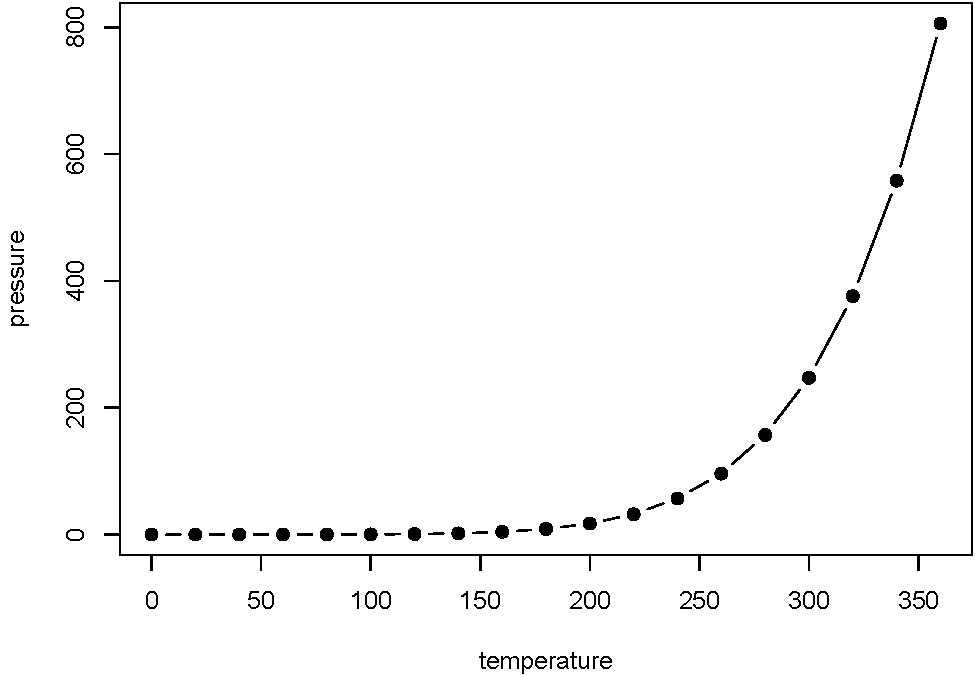
\includegraphics{ucas_zh_files/figure-latex/unnamed-chunk-1-1.pdf}

当然,在使用LaTex制作论文并插入图片时,你几乎不可避免的会遇到图片浮动的问题,即图片可能会出现在文章的其他位置。如果你不常使用LaTex并且不希望这种情况发生,你应该注意图片的浮动问题,通过修改图片的尺寸来解决这个问题。

和前面的定理环境相似,你也可以通过chunk option对代码块设定标签并在后面进行引用,同时你还可以使用更多knitr中R code chunk的设定来对图片进行更好的控制。

\begin{Shaded}
\begin{Highlighting}[]
\KeywordTok{par}\NormalTok{(}\DataTypeTok{mar =} \KeywordTok{c}\NormalTok{(}\DecValTok{4}\NormalTok{, }\DecValTok{4}\NormalTok{, }\FloatTok{0.1}\NormalTok{, }\FloatTok{0.1}\NormalTok{))}
\KeywordTok{plot}\NormalTok{(pressure, }\DataTypeTok{pch =} \DecValTok{19}\NormalTok{, }\DataTypeTok{type =} \StringTok{"b"}\NormalTok{)}
\end{Highlighting}
\end{Shaded}

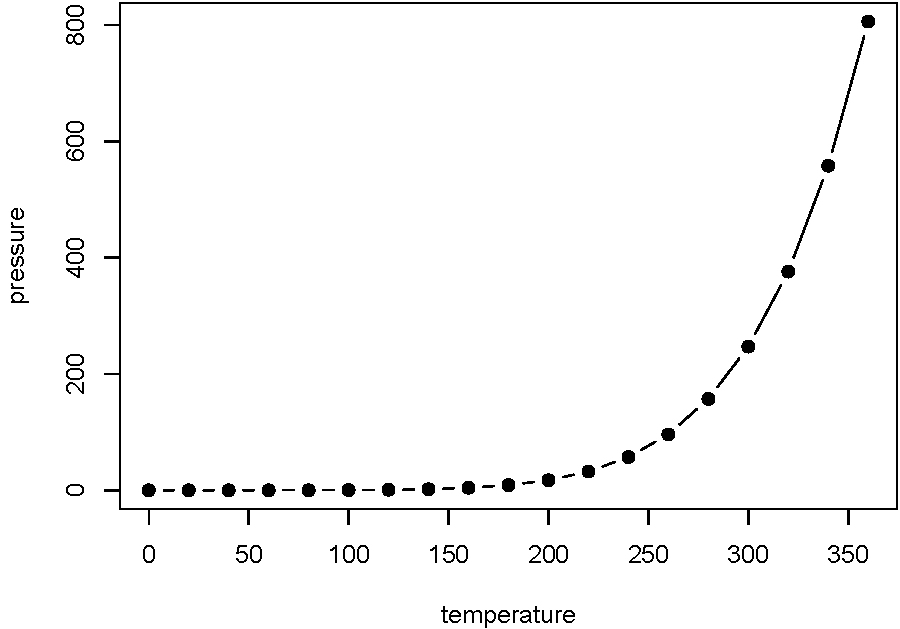
\includegraphics{ucas_zh_files/figure-latex/pressure-1.pdf}
在输出这个图片时,我们使用了\texttt{fig.cap}来设定图片标题,用\texttt{fig.width}设定了图片的宽度,用\texttt{fig.asp\ =\ 0.7}设定图片的长宽比例固定在0.7,\texttt{fig.aligin\ =\ \textquotesingle{}center\textquotesingle{}}令图片居中。你还可以使用其他的R chunk option来对图片进行设置。更多的设置可以见\href{https://yihui.name/knitr/options/\#plots}{option-plots}。

\hypertarget{section-4}{%
\section{插入本地图片}\label{section-4}}

在使用Rmarkdown的过程中,你同样可以使用markdown/LaTex/html的语法插入本地图片,不过我们更推荐你使用\texttt{knitr::include\_graphics()},主要原因有:

\begin{enumerate}
\def\labelenumi{\arabic{enumi}.}
\tightlist
\item
  你不需要担心文档的输出格式,\texttt{knitr::include\_graphics()}可以根据你的文档输出格式来自适应的选择输出函数\texttt{!{[}{]}()}(markdown)、\texttt{\textbackslash{}includegraphics}(LaTex)或是其他的输出函数;
\item
  在使用knitr函数的过程中,你可以像上面一样轻松的使用chunk option来对图片进行设定和约束;
\item
  当输出PDF文件时,\texttt{include\_graphics()}可以自动帮助你将原有的png或jpg图片替换为pdf格式,可以在输出pdf文档时获得更好的体验。
\end{enumerate}

\hypertarget{section-5}{%
\section{表格}\label{section-5}}

在bookdown中,你可以使用markdown语法的表格,或者LaTex语法的表格,或者使用R中的一些制表的辅助包、辅助函数如\texttt{knitr::kable()}、\texttt{huxtable}或\texttt{xtable}等。使用\texttt{kable},你可以轻松的将R中的数据框输出为html或LaTex制式的表格,例如:

\begin{Shaded}
\begin{Highlighting}[]
\NormalTok{knitr}\OperatorTok{::}\KeywordTok{kable}\NormalTok{(}
  \KeywordTok{head}\NormalTok{(mtcars[, }\DecValTok{1}\OperatorTok{:}\DecValTok{8}\NormalTok{], }\DecValTok{10}\NormalTok{), }\DataTypeTok{booktabs =} \OtherTok{TRUE}\NormalTok{,}
  \DataTypeTok{caption =} \StringTok{'kable()输出的一个表'}
\NormalTok{)}
\end{Highlighting}
\end{Shaded}

\begin{table}[t]

\caption{\label{tab:kb-table}kable()输出的一个表}
\centering
\begin{tabular}{lrrrrrrrr}
\toprule
  & mpg & cyl & disp & hp & drat & wt & qsec & vs\\
\midrule
Mazda RX4 & 21.0 & 6 & 160.0 & 110 & 3.90 & 2.620 & 16.46 & 0\\
Mazda RX4 Wag & 21.0 & 6 & 160.0 & 110 & 3.90 & 2.875 & 17.02 & 0\\
Datsun 710 & 22.8 & 4 & 108.0 & 93 & 3.85 & 2.320 & 18.61 & 1\\
Hornet 4 Drive & 21.4 & 6 & 258.0 & 110 & 3.08 & 3.215 & 19.44 & 1\\
Hornet Sportabout & 18.7 & 8 & 360.0 & 175 & 3.15 & 3.440 & 17.02 & 0\\
\addlinespace
Valiant & 18.1 & 6 & 225.0 & 105 & 2.76 & 3.460 & 20.22 & 1\\
Duster 360 & 14.3 & 8 & 360.0 & 245 & 3.21 & 3.570 & 15.84 & 0\\
Merc 240D & 24.4 & 4 & 146.7 & 62 & 3.69 & 3.190 & 20.00 & 1\\
Merc 230 & 22.8 & 4 & 140.8 & 95 & 3.92 & 3.150 & 22.90 & 1\\
Merc 280 & 19.2 & 6 & 167.6 & 123 & 3.92 & 3.440 & 18.30 & 1\\
\bottomrule
\end{tabular}
\end{table}

当然,如果熟悉markdown,你也可以使用makrdown语法的表格

\begin{verbatim}
Table: A simple table in Markdown.

 Sepal.Length   Sepal.Width   Petal.Length   Petal.Width
-------------  ------------  -------------  ------------
          5.1           3.5            1.4           0.2
          4.9           3.0            1.4           0.2
          4.7           3.2            1.3           0.2
          4.6           3.1            1.5           0.2
          5.0           3.6            1.4           0.2
          5.4           3.9            1.7           0.4
\end{verbatim}

基于bookdown的便利性,你也可以像引用图片一样方便的引用这些表格。

\hypertarget{section-6}{%
\subsection{回归结果}\label{section-6}}

对于回归分析的结果,你可以调用\href{}{\texttt{huxtable}}包来轻松的进行学术化的制表,甚至可以对多个回归方程轻松的联合制表。

\begin{Shaded}
\begin{Highlighting}[]
\KeywordTok{library}\NormalTok{(dplyr)}
\KeywordTok{library}\NormalTok{(huxtable)}
\KeywordTok{data}\NormalTok{(diamonds, }\DataTypeTok{package =} \StringTok{'ggplot2'}\NormalTok{)}
\NormalTok{lm1 <-}\StringTok{ }\KeywordTok{lm}\NormalTok{(price }\OperatorTok{~}\StringTok{ }\NormalTok{carat }\OperatorTok{+}\StringTok{ }\NormalTok{depth, diamonds)}
\NormalTok{lm2 <-}\StringTok{ }\KeywordTok{lm}\NormalTok{(price }\OperatorTok{~}\StringTok{ }\NormalTok{depth }\OperatorTok{+}\StringTok{ }\KeywordTok{factor}\NormalTok{(color, }\DataTypeTok{ordered =} \OtherTok{FALSE}\NormalTok{), diamonds)}
\NormalTok{lm3 <-}\StringTok{ }\KeywordTok{lm}\NormalTok{(}\KeywordTok{log}\NormalTok{(price) }\OperatorTok{~}\StringTok{ }\NormalTok{carat }\OperatorTok{+}\StringTok{ }\NormalTok{depth, diamonds)}
\end{Highlighting}
\end{Shaded}

\begin{Shaded}
\begin{Highlighting}[]
\NormalTok{color_names <-}\StringTok{ }\KeywordTok{paste0}\NormalTok{(}\StringTok{'factor(color, ordered = FALSE)'}\NormalTok{, LETTERS[}\DecValTok{5}\OperatorTok{:}\DecValTok{10}\NormalTok{])}
\KeywordTok{names}\NormalTok{(color_names) <-}\StringTok{ }\KeywordTok{paste}\NormalTok{(}\StringTok{'Color:'}\NormalTok{, LETTERS[}\DecValTok{5}\OperatorTok{:}\DecValTok{10}\NormalTok{])}

\KeywordTok{huxreg}\NormalTok{(lm1, lm2, lm3, }
  \DataTypeTok{coefs =} \KeywordTok{c}\NormalTok{(}\StringTok{'Carat'}\NormalTok{ =}\StringTok{ 'carat'}\NormalTok{, }\StringTok{'Depth'}\NormalTok{ =}\StringTok{ 'depth'}\NormalTok{, color_names)) }\OperatorTok\StringTok{ }
\StringTok{  }\KeywordTok{theme_article}\NormalTok{()}
\end{Highlighting}
\end{Shaded}

 
  \providecommand{\huxb}[2]{\arrayrulecolor[RGB]{#1}\global\arrayrulewidth=#2pt}
  \providecommand{\huxvb}[2]{\color[RGB]{#1}\vrule width #2pt}
  \providecommand{\huxtpad}[1]{\rule{0pt}{\baselineskip+#1}}
  \providecommand{\huxbpad}[1]{\rule[-#1]{0pt}{#1}}

\begin{table}[h]
\centering
\begin{threeparttable}
\begin{tabularx}{0.5\textwidth}{p{0.125\textwidth} p{0.125\textwidth} p{0.125\textwidth} p{0.125\textwidth}}


\hhline{>{\huxb{0, 0, 0}{1}}->{\huxb{0, 0, 0}{1}}->{\huxb{0, 0, 0}{1}}->{\huxb{0, 0, 0}{1}}-}
\arrayrulecolor{black}

\multicolumn{1}{!{\huxvb{0, 0, 0}{0}}c!{\huxvb{0, 0, 0}{0}}}{\huxtpad{4pt}\centering \textbf{}\huxbpad{4pt}} &
\multicolumn{1}{c!{\huxvb{0, 0, 0}{0}}}{\huxtpad{4pt}\centering \textbf{(1)}\huxbpad{4pt}} &
\multicolumn{1}{c!{\huxvb{0, 0, 0}{0}}}{\huxtpad{4pt}\centering \textbf{(2)}\huxbpad{4pt}} &
\multicolumn{1}{c!{\huxvb{0, 0, 0}{0}}}{\huxtpad{4pt}\centering \textbf{(3)}\huxbpad{4pt}} \tabularnewline[-0.5pt]


\hhline{>{\huxb{0, 0, 0}{1}}->{\huxb{0, 0, 0}{1}}->{\huxb{0, 0, 0}{1}}->{\huxb{0, 0, 0}{1}}-}
\arrayrulecolor{black}

\multicolumn{1}{!{\huxvb{0, 0, 0}{0}}l!{\huxvb{0, 0, 0}{0}}}{\huxtpad{4pt}\raggedright \textbf{Carat}\huxbpad{4pt}} &
\multicolumn{1}{r!{\huxvb{0, 0, 0}{0}}}{\huxtpad{4pt}\raggedleft 7765.141 ***\huxbpad{4pt}} &
\multicolumn{1}{r!{\huxvb{0, 0, 0}{0}}}{\huxtpad{4pt}\raggedleft ~~~~~~~~\huxbpad{4pt}} &
\multicolumn{1}{r!{\huxvb{0, 0, 0}{0}}}{\huxtpad{4pt}\raggedleft 1.971 ***\huxbpad{4pt}} \tabularnewline[-0.5pt]


\hhline{}
\arrayrulecolor{black}

\multicolumn{1}{!{\huxvb{0, 0, 0}{0}}l!{\huxvb{0, 0, 0}{0}}}{\huxtpad{4pt}\raggedright \textbf{}\huxbpad{4pt}} &
\multicolumn{1}{r!{\huxvb{0, 0, 0}{0}}}{\huxtpad{4pt}\raggedleft (14.009)~~~\huxbpad{4pt}} &
\multicolumn{1}{r!{\huxvb{0, 0, 0}{0}}}{\huxtpad{4pt}\raggedleft ~~~~~~~~\huxbpad{4pt}} &
\multicolumn{1}{r!{\huxvb{0, 0, 0}{0}}}{\huxtpad{4pt}\raggedleft (0.004)~~~\huxbpad{4pt}} \tabularnewline[-0.5pt]


\hhline{}
\arrayrulecolor{black}

\multicolumn{1}{!{\huxvb{0, 0, 0}{0}}l!{\huxvb{0, 0, 0}{0}}}{\huxtpad{4pt}\raggedright \textbf{Depth}\huxbpad{4pt}} &
\multicolumn{1}{r!{\huxvb{0, 0, 0}{0}}}{\huxtpad{4pt}\raggedleft -102.165 ***\huxbpad{4pt}} &
\multicolumn{1}{r!{\huxvb{0, 0, 0}{0}}}{\huxtpad{4pt}\raggedleft -53.835 ***\huxbpad{4pt}} &
\multicolumn{1}{r!{\huxvb{0, 0, 0}{0}}}{\huxtpad{4pt}\raggedleft -0.018 ***\huxbpad{4pt}} \tabularnewline[-0.5pt]


\hhline{}
\arrayrulecolor{black}

\multicolumn{1}{!{\huxvb{0, 0, 0}{0}}l!{\huxvb{0, 0, 0}{0}}}{\huxtpad{4pt}\raggedright \textbf{}\huxbpad{4pt}} &
\multicolumn{1}{r!{\huxvb{0, 0, 0}{0}}}{\huxtpad{4pt}\raggedleft (4.635)~~~\huxbpad{4pt}} &
\multicolumn{1}{r!{\huxvb{0, 0, 0}{0}}}{\huxtpad{4pt}\raggedleft (11.815)~~~\huxbpad{4pt}} &
\multicolumn{1}{r!{\huxvb{0, 0, 0}{0}}}{\huxtpad{4pt}\raggedleft (0.001)~~~\huxbpad{4pt}} \tabularnewline[-0.5pt]


\hhline{}
\arrayrulecolor{black}

\multicolumn{1}{!{\huxvb{0, 0, 0}{0}}l!{\huxvb{0, 0, 0}{0}}}{\huxtpad{4pt}\raggedright \textbf{Color: E}\huxbpad{4pt}} &
\multicolumn{1}{r!{\huxvb{0, 0, 0}{0}}}{\huxtpad{4pt}\raggedleft ~~~~~~~~\huxbpad{4pt}} &
\multicolumn{1}{r!{\huxvb{0, 0, 0}{0}}}{\huxtpad{4pt}\raggedleft -95.142~~~~\huxbpad{4pt}} &
\multicolumn{1}{r!{\huxvb{0, 0, 0}{0}}}{\huxtpad{4pt}\raggedleft ~~~~~~~~\huxbpad{4pt}} \tabularnewline[-0.5pt]


\hhline{}
\arrayrulecolor{black}

\multicolumn{1}{!{\huxvb{0, 0, 0}{0}}l!{\huxvb{0, 0, 0}{0}}}{\huxtpad{4pt}\raggedright \textbf{}\huxbpad{4pt}} &
\multicolumn{1}{r!{\huxvb{0, 0, 0}{0}}}{\huxtpad{4pt}\raggedleft ~~~~~~~~\huxbpad{4pt}} &
\multicolumn{1}{r!{\huxvb{0, 0, 0}{0}}}{\huxtpad{4pt}\raggedleft (62.037)~~~\huxbpad{4pt}} &
\multicolumn{1}{r!{\huxvb{0, 0, 0}{0}}}{\huxtpad{4pt}\raggedleft ~~~~~~~~\huxbpad{4pt}} \tabularnewline[-0.5pt]


\hhline{}
\arrayrulecolor{black}

\multicolumn{1}{!{\huxvb{0, 0, 0}{0}}l!{\huxvb{0, 0, 0}{0}}}{\huxtpad{4pt}\raggedright \textbf{Color: F}\huxbpad{4pt}} &
\multicolumn{1}{r!{\huxvb{0, 0, 0}{0}}}{\huxtpad{4pt}\raggedleft ~~~~~~~~\huxbpad{4pt}} &
\multicolumn{1}{r!{\huxvb{0, 0, 0}{0}}}{\huxtpad{4pt}\raggedleft 554.742 ***\huxbpad{4pt}} &
\multicolumn{1}{r!{\huxvb{0, 0, 0}{0}}}{\huxtpad{4pt}\raggedleft ~~~~~~~~\huxbpad{4pt}} \tabularnewline[-0.5pt]


\hhline{}
\arrayrulecolor{black}

\multicolumn{1}{!{\huxvb{0, 0, 0}{0}}l!{\huxvb{0, 0, 0}{0}}}{\huxtpad{4pt}\raggedright \textbf{}\huxbpad{4pt}} &
\multicolumn{1}{r!{\huxvb{0, 0, 0}{0}}}{\huxtpad{4pt}\raggedleft ~~~~~~~~\huxbpad{4pt}} &
\multicolumn{1}{r!{\huxvb{0, 0, 0}{0}}}{\huxtpad{4pt}\raggedleft (62.374)~~~\huxbpad{4pt}} &
\multicolumn{1}{r!{\huxvb{0, 0, 0}{0}}}{\huxtpad{4pt}\raggedleft ~~~~~~~~\huxbpad{4pt}} \tabularnewline[-0.5pt]


\hhline{}
\arrayrulecolor{black}

\multicolumn{1}{!{\huxvb{0, 0, 0}{0}}l!{\huxvb{0, 0, 0}{0}}}{\huxtpad{4pt}\raggedright \textbf{Color: G}\huxbpad{4pt}} &
\multicolumn{1}{r!{\huxvb{0, 0, 0}{0}}}{\huxtpad{4pt}\raggedleft ~~~~~~~~\huxbpad{4pt}} &
\multicolumn{1}{r!{\huxvb{0, 0, 0}{0}}}{\huxtpad{4pt}\raggedleft 832.357 ***\huxbpad{4pt}} &
\multicolumn{1}{r!{\huxvb{0, 0, 0}{0}}}{\huxtpad{4pt}\raggedleft ~~~~~~~~\huxbpad{4pt}} \tabularnewline[-0.5pt]


\hhline{}
\arrayrulecolor{black}

\multicolumn{1}{!{\huxvb{0, 0, 0}{0}}l!{\huxvb{0, 0, 0}{0}}}{\huxtpad{4pt}\raggedright \textbf{}\huxbpad{4pt}} &
\multicolumn{1}{r!{\huxvb{0, 0, 0}{0}}}{\huxtpad{4pt}\raggedleft ~~~~~~~~\huxbpad{4pt}} &
\multicolumn{1}{r!{\huxvb{0, 0, 0}{0}}}{\huxtpad{4pt}\raggedleft (60.338)~~~\huxbpad{4pt}} &
\multicolumn{1}{r!{\huxvb{0, 0, 0}{0}}}{\huxtpad{4pt}\raggedleft ~~~~~~~~\huxbpad{4pt}} \tabularnewline[-0.5pt]


\hhline{}
\arrayrulecolor{black}

\multicolumn{1}{!{\huxvb{0, 0, 0}{0}}l!{\huxvb{0, 0, 0}{0}}}{\huxtpad{4pt}\raggedright \textbf{Color: H}\huxbpad{4pt}} &
\multicolumn{1}{r!{\huxvb{0, 0, 0}{0}}}{\huxtpad{4pt}\raggedleft ~~~~~~~~\huxbpad{4pt}} &
\multicolumn{1}{r!{\huxvb{0, 0, 0}{0}}}{\huxtpad{4pt}\raggedleft 1324.183 ***\huxbpad{4pt}} &
\multicolumn{1}{r!{\huxvb{0, 0, 0}{0}}}{\huxtpad{4pt}\raggedleft ~~~~~~~~\huxbpad{4pt}} \tabularnewline[-0.5pt]


\hhline{}
\arrayrulecolor{black}

\multicolumn{1}{!{\huxvb{0, 0, 0}{0}}l!{\huxvb{0, 0, 0}{0}}}{\huxtpad{4pt}\raggedright \textbf{}\huxbpad{4pt}} &
\multicolumn{1}{r!{\huxvb{0, 0, 0}{0}}}{\huxtpad{4pt}\raggedleft ~~~~~~~~\huxbpad{4pt}} &
\multicolumn{1}{r!{\huxvb{0, 0, 0}{0}}}{\huxtpad{4pt}\raggedleft (64.296)~~~\huxbpad{4pt}} &
\multicolumn{1}{r!{\huxvb{0, 0, 0}{0}}}{\huxtpad{4pt}\raggedleft ~~~~~~~~\huxbpad{4pt}} \tabularnewline[-0.5pt]


\hhline{}
\arrayrulecolor{black}

\multicolumn{1}{!{\huxvb{0, 0, 0}{0}}l!{\huxvb{0, 0, 0}{0}}}{\huxtpad{4pt}\raggedright \textbf{Color: I}\huxbpad{4pt}} &
\multicolumn{1}{r!{\huxvb{0, 0, 0}{0}}}{\huxtpad{4pt}\raggedleft ~~~~~~~~\huxbpad{4pt}} &
\multicolumn{1}{r!{\huxvb{0, 0, 0}{0}}}{\huxtpad{4pt}\raggedleft 1929.902 ***\huxbpad{4pt}} &
\multicolumn{1}{r!{\huxvb{0, 0, 0}{0}}}{\huxtpad{4pt}\raggedleft ~~~~~~~~\huxbpad{4pt}} \tabularnewline[-0.5pt]


\hhline{}
\arrayrulecolor{black}

\multicolumn{1}{!{\huxvb{0, 0, 0}{0}}l!{\huxvb{0, 0, 0}{0}}}{\huxtpad{4pt}\raggedright \textbf{}\huxbpad{4pt}} &
\multicolumn{1}{r!{\huxvb{0, 0, 0}{0}}}{\huxtpad{4pt}\raggedleft ~~~~~~~~\huxbpad{4pt}} &
\multicolumn{1}{r!{\huxvb{0, 0, 0}{0}}}{\huxtpad{4pt}\raggedleft (71.561)~~~\huxbpad{4pt}} &
\multicolumn{1}{r!{\huxvb{0, 0, 0}{0}}}{\huxtpad{4pt}\raggedleft ~~~~~~~~\huxbpad{4pt}} \tabularnewline[-0.5pt]


\hhline{}
\arrayrulecolor{black}

\multicolumn{1}{!{\huxvb{0, 0, 0}{0}}l!{\huxvb{0, 0, 0}{0}}}{\huxtpad{4pt}\raggedright \textbf{Color: J}\huxbpad{4pt}} &
\multicolumn{1}{r!{\huxvb{0, 0, 0}{0}}}{\huxtpad{4pt}\raggedleft ~~~~~~~~\huxbpad{4pt}} &
\multicolumn{1}{r!{\huxvb{0, 0, 0}{0}}}{\huxtpad{4pt}\raggedleft 2164.044 ***\huxbpad{4pt}} &
\multicolumn{1}{r!{\huxvb{0, 0, 0}{0}}}{\huxtpad{4pt}\raggedleft ~~~~~~~~\huxbpad{4pt}} \tabularnewline[-0.5pt]


\hhline{}
\arrayrulecolor{black}

\multicolumn{1}{!{\huxvb{0, 0, 0}{0}}l!{\huxvb{0, 0, 0}{0}}}{\huxtpad{4pt}\raggedright \textbf{}\huxbpad{4pt}} &
\multicolumn{1}{r!{\huxvb{0, 0, 0}{0}}}{\huxtpad{4pt}\raggedleft ~~~~~~~~\huxbpad{4pt}} &
\multicolumn{1}{r!{\huxvb{0, 0, 0}{0}}}{\huxtpad{4pt}\raggedleft (88.144)~~~\huxbpad{4pt}} &
\multicolumn{1}{r!{\huxvb{0, 0, 0}{0}}}{\huxtpad{4pt}\raggedleft ~~~~~~~~\huxbpad{4pt}} \tabularnewline[-0.5pt]


\hhline{}
\arrayrulecolor{black}

\multicolumn{1}{!{\huxvb{0, 0, 0}{0}}l!{\huxvb{0, 0, 0}{0}}}{\huxtpad{4pt}\raggedright \textbf{N}\huxbpad{4pt}} &
\multicolumn{1}{r!{\huxvb{0, 0, 0}{0}}}{\huxtpad{4pt}\raggedleft 53940~~~~~~~~\huxbpad{4pt}} &
\multicolumn{1}{r!{\huxvb{0, 0, 0}{0}}}{\huxtpad{4pt}\raggedleft 53940~~~~~~~~\huxbpad{4pt}} &
\multicolumn{1}{r!{\huxvb{0, 0, 0}{0}}}{\huxtpad{4pt}\raggedleft 53940~~~~~~~~\huxbpad{4pt}} \tabularnewline[-0.5pt]


\hhline{}
\arrayrulecolor{black}

\multicolumn{1}{!{\huxvb{0, 0, 0}{0}}l!{\huxvb{0, 0, 0}{0}}}{\huxtpad{4pt}\raggedright \textbf{R2}\huxbpad{4pt}} &
\multicolumn{1}{r!{\huxvb{0, 0, 0}{0}}}{\huxtpad{4pt}\raggedleft 0.851~~~~\huxbpad{4pt}} &
\multicolumn{1}{r!{\huxvb{0, 0, 0}{0}}}{\huxtpad{4pt}\raggedleft 0.032~~~~\huxbpad{4pt}} &
\multicolumn{1}{r!{\huxvb{0, 0, 0}{0}}}{\huxtpad{4pt}\raggedleft 0.847~~~~\huxbpad{4pt}} \tabularnewline[-0.5pt]


\hhline{}
\arrayrulecolor{black}

\multicolumn{1}{!{\huxvb{0, 0, 0}{0}}l!{\huxvb{0, 0, 0}{0}}}{\huxtpad{4pt}\raggedright \textbf{logLik}\huxbpad{4pt}} &
\multicolumn{1}{r!{\huxvb{0, 0, 0}{0}}}{\huxtpad{4pt}\raggedleft -472488.441~~~~\huxbpad{4pt}} &
\multicolumn{1}{r!{\huxvb{0, 0, 0}{0}}}{\huxtpad{4pt}\raggedleft -522908.139~~~~\huxbpad{4pt}} &
\multicolumn{1}{r!{\huxvb{0, 0, 0}{0}}}{\huxtpad{4pt}\raggedleft -26617.649~~~~\huxbpad{4pt}} \tabularnewline[-0.5pt]


\hhline{}
\arrayrulecolor{black}

\multicolumn{1}{!{\huxvb{0, 0, 0}{0}}l!{\huxvb{0, 0, 0}{0}}}{\huxtpad{4pt}\raggedright \textbf{AIC}\huxbpad{4pt}} &
\multicolumn{1}{r!{\huxvb{0, 0, 0}{0}}}{\huxtpad{4pt}\raggedleft 944984.882~~~~\huxbpad{4pt}} &
\multicolumn{1}{r!{\huxvb{0, 0, 0}{0}}}{\huxtpad{4pt}\raggedleft 1045834.277~~~~\huxbpad{4pt}} &
\multicolumn{1}{r!{\huxvb{0, 0, 0}{0}}}{\huxtpad{4pt}\raggedleft 53243.298~~~~\huxbpad{4pt}} \tabularnewline[-0.5pt]


\hhline{}
\arrayrulecolor{black}

\multicolumn{4}{!{\huxvb{0, 0, 0}{0}}p{0.5\textwidth+6\tabcolsep}!{\huxvb{0, 0, 0}{0}}}{\parbox[b]{0.5\textwidth+6\tabcolsep-4pt-4pt}{\huxtpad{4pt}\raggedright \textbf{ *** p $<$ 0.001;  ** p $<$ 0.01;  * p $<$ 0.05.}\huxbpad{4pt}}} \tabularnewline[-0.5pt]


\hhline{>{\huxb{0, 0, 0}{1}}->{\huxb{0, 0, 0}{1}}->{\huxb{0, 0, 0}{1}}->{\huxb{0, 0, 0}{1}}-}
\arrayrulecolor{black}
\end{tabularx}\end{threeparttable}


\end{table}
 

更多的关于\texttt{huxreg()}的用法可以见\href{https://hughjonesd.github.io/huxtable/huxreg.html}{这里}。

\hypertarget{section-7}{%
\section{交叉引用与引文}\label{section-7}}

与前面的引用图标、公式、定理的方法相同,你也可以用\texttt{\textbackslash{}@ref(label)}来引用章节标题,如果是英文标题,pandoc将自动为之分配一个标签,如章Reference 将拥有一个标签reference。如果是中文标题,可以考虑使用Peng Zhao开发的包\href{https://github.com/pzhaonet/pinyin}{\texttt{pinyin}},它可以自动给中文章节分配一个与其拼音拼写对应的标签。

不过这可能会导致某个章节的标签过长,所以我们还是建议你自己为每个章节定制标签,在每个章节后添加\{\#ID\},ID即为本章的标签。

\hypertarget{bibtex}{%
\subsection{bibtex与文献引用}\label{bibtex}}

为了方便的引用和排列参考文献,你应该使用bibtex来对参考文献进行管理。pandoc可以利用\href{https://github.com/jgm/pandoc-citeproc}{\texttt{pandoc-citeproc}}单元来处理文献引用的问题,当输出格式为LaTex时,利用BibTex可以更好的处理参考文献。

一个BibTex database文件时一个纯文本文件(文件拓展名为\texttt{.bib}),其中一个书目条目(bibliography entry)的主要内容应该如:

\begin{verbatim}

@Manual{R-base,
  title = {R: A Language and Environment for Statistical
    Computing},
  author = {{R Core Team}},
  organization = {R Foundation for Statistical Computing},
  address = {Vienna, Austria},
  year = {2016},
  url = {https://www.R-project.org/},
}
\end{verbatim}

每一个书目条目以\texttt{@type\{}起始,其中type包括\texttt{article}、\texttt{book}、\texttt{Manual}等类型,然后每个书目条目中有一个引用关键字,如上面的\texttt{R-base},你可以使用\texttt{@R-base}
或\texttt{{[}@R-base{]}}来引用它,后者将会在括号中引用文献,如{[}@R-base{]}。

同时在\texttt{knitr}中还有一个辅助函数\texttt{knitr::write\_bib()}可以帮助你引用在写论文时使用到的包。例如:

\begin{Shaded}
\begin{Highlighting}[]
\NormalTok{knitr}\OperatorTok{::}\KeywordTok{write_bib}\NormalTok{(}\KeywordTok{c}\NormalTok{(}\StringTok{"knitr"}\NormalTok{, }\StringTok{"stringr"}\NormalTok{), }\StringTok{"bib/Rpackage.bib"}\NormalTok{, }\DataTypeTok{width =} \DecValTok{60}\NormalTok{)}
\end{Highlighting}
\end{Shaded}

会生成一个名为\texttt{Rpackage}内容如下的\texttt{.bib}文件

\begin{Shaded}
\begin{Highlighting}[]
\VariableTok{@Manual}\NormalTok{\{}\OtherTok{R}\NormalTok{-}\OtherTok{knitr}\NormalTok{,}
  \DataTypeTok{title}\NormalTok{ = \{knitr: A General-Purpose Package for Dynamic Report}
\NormalTok{    Generation in R\},}
  \DataTypeTok{author}\NormalTok{ = \{Yihui Xie\},}
  \DataTypeTok{year}\NormalTok{ = \{2018\},}
  \DataTypeTok{note}\NormalTok{ = \{R package version 1.20.22\},}
  \DataTypeTok{url}\NormalTok{ = \{https://yihui.name/knitr/\},}
\NormalTok{\}}
\VariableTok{@Manual}\NormalTok{\{}\OtherTok{R}\NormalTok{-}\OtherTok{stringr}\NormalTok{,}
  \DataTypeTok{title}\NormalTok{ = \{stringr: Simple, Consistent Wrappers for Common}
\NormalTok{    String Operations\},}
  \DataTypeTok{author}\NormalTok{ = \{Hadley Wickham\},}
  \DataTypeTok{year}\NormalTok{ = \{2018\},}
  \DataTypeTok{note}\NormalTok{ = \{R package version 1.3.1\},}
  \DataTypeTok{url}\NormalTok{ = \{https://CRAN.R-project.org/package=stringr\},}
\NormalTok{\}}
\end{Highlighting}
\end{Shaded}

如果你有一个或多个bib文件,你需要在index.Rmd的YAML metadata(即文档开头一对\texttt{-\/-\/-}中间的内容)中的\texttt{bibliography}中引用它们,如:

\begin{verbatim}
---
bibliography: [bib/bib.bib, bib/Rpackage.bib]
---
\end{verbatim}

然后你就可以在文章中引用添加在\texttt{.bib}中的文献,如{[}@R-knitr{]}。

\hypertarget{tinytex}{%
\chapter{使用TinyTex}\label{tinytex}}

为了节省电脑的硬盘空间,同时还能够方便的使用LaTex的编译,避免在使用Rmarkdown的过程中遇到LaTex包缺失的问题,我们建议你使用\href{https://yihui.name/tinytex/cn/}{TinyTex},它是一个瘦身版的Tex Live,去掉了其中没有用处的文档和源代码,使用了Tex Live的自动化安装方式。

\hypertarget{tinytex-1}{%
\section{安装TinyTex}\label{tinytex-1}}

对于R用户,你可以方便的安装TinyTex,只需要运行以下指令然后等待几分钟(windows用户的安装过程中可能会弹出两次错误对话框,点击确定即可)

\begin{Shaded}
\begin{Highlighting}[]
\CommentTok{# install.packages('remotes')}
\NormalTok{remotes}\OperatorTok{::}\KeywordTok{install_github}\NormalTok{(}\StringTok{'yihui/tinytex'}\NormalTok{)}
\NormalTok{tinytex}\OperatorTok{::}\KeywordTok{install_tinytex}\NormalTok{()}
\end{Highlighting}
\end{Shaded}

注意,在一个电脑上安装多个LaTex套件可能会出现冲突,所以在安装之前,建议将电脑上的MikTex、Tex Live等卸载。在整个TinyTex安装完成之后,你可以运行

\begin{Shaded}
\begin{Highlighting}[]
\NormalTok{tinytex}\OperatorTok{::}\KeywordTok{is_tinytex_install}\NormalTok{()}
\end{Highlighting}
\end{Shaded}

来检查TinyTex是否安装完成。

\hypertarget{tinytex-2}{%
\section{使用TinyTex}\label{tinytex-2}}

理论上而言,在TinyTex安装完成后,它可以自动安装你在使用不同Rmarkdown文档中依赖的LaTex包,你在第一次编译本文档时就可以体会到它的方便之处。当然我们还是不能排除TinyTex出现bug的可能性,所以你需要对它的基本函数的使用有一些了解。

\hypertarget{section-8}{%
\subsection{进行调试}\label{section-8}}

在使用Rmarkdown的过程中你可能会遇到一些来自LaTex的错误,如果你不想在每次报错后都阅读完成的log文件,你可以在文档中插入代码块

\begin{Shaded}
\begin{Highlighting}[]

\end{Highlighting}
\end{Shaded}

然后在Rstudio中获取错误信息,并根据错误做进一步的调整。

\hypertarget{section-9}{%
\subsection{手动安装依赖包}\label{section-9}}

当然,你也可能会遇到一些情况,TinyTex没有自动安装编译所依赖的包,这时你需要手动进行安装。通常,你可能会根据错误信息判断出缺失的文件\texttt{xxx.sty},然后你可以在R中调用\texttt{tlmgr\_search()}寻找包含\texttt{xxx.sty}的LaTex包,然后使用\texttt{tlmgr\_install()}对缺失的包进行下载。

同样存在一些可能,你需要更新TeX Live,你需要调用\texttt{tlmgr\_update()}。

\begin{Shaded}
\begin{Highlighting}[]
\KeywordTok{library}\NormalTok{(tinytex)}
\KeywordTok{tlmgr_search}\NormalTok{(}\StringTok{'framed.sty'}\NormalTok{)  }\CommentTok{# 搜索包含 framed.sty 文件的 LaTeX 包}
\KeywordTok{tlmgr_install}\NormalTok{(}\StringTok{'framed'}\NormalTok{)     }\CommentTok{# 安装 framed 包}
\KeywordTok{tlmgr_update}\NormalTok{()              }\CommentTok{# 更新 TeX Live}
\end{Highlighting}
\end{Shaded}

\hypertarget{section-10}{%
\chapter{致谢}\label{section-10}}

本模板源自 mohuangrui/ucasthesis \LaTeX\{\} 模板\footnote{\url{https://gitlab.com/mohuangrui/ucasthesis}}。感谢!

首先要感谢yihui,毕竟创世神;还有zhao peng,他改造了ucas毕业论文的LaTex模板使之适用于bookdown,并在我准备对模板继续改造时提供了非常关键的帮助。

追本溯源的话,应该还有pandoc,甚至Ctex的开发者,就不多言了。

\hypertarget{section-11}{%
\chapter*{参考文献}\label{section-11}}
\addcontentsline{toc}{chapter}{参考文献}

\setlength{\bibsep}{0ex}
\bibliography{bib/bib.bib, bib/Rpackage.bib}

\appendix

\hypertarget{section-12}{%
\chapter{中南财经政法大学本科生毕业论文规范}\label{section-12}}

\raggedbottom

为了进一步规范我校本科生毕业论文(设计)的撰写工作,提高论文撰写质量与规范化水平,现根据《中南财经政法大学本科生毕业论文(设计)管理办法》的要求,参照中国国家标准标准化管理委员会所发布的《科学技术报告、学位论文和学术论文的编写格式》(GB/T7713-1987)和《文后参考文献著录规则》(GB/T7714-2005)等标准,以及中华人民共和国新闻署和中国国家语言文字工作委员会等机构发布的相关规则,结合我校学科结构上的特点,特制定本规范。

\hypertarget{section-13}{%
\section{毕业论文(设计)内容及要求}\label{section-13}}

毕业论文(设计)应包括以下项目:(1)封面;(2)作者声明;(3)论文(设计)题目及署名;(4)中外(英)文摘要及关键词;(5)目录;(6)正文;(7)注释;(8)主要参考文献;(9)附录(非必选项);(10)后记(非必选项)。以上各项目的基本内容与要求如下:

\hypertarget{section-14}{%
\subsection{封面}\label{section-14}}

\textbf{封面信息。} 封面信息包括学校名称与本科生毕业论文(设计)的全称、毕业论文标题(含毕业设计,以下简称论文)、学生个人信息、指导老师信息,以及论文完成(提交答辩)时间等。

\textbf{封面格式。} 封面格式由学校统一设计、印制后发放。封面上的题目、姓名、学号、班级、年级、专业、院系、指导教师姓名及职称等内容,以及论文完成时间。封面最好是打印填列,所有项目填列的内容均须排列整齐、美观。

\hypertarget{section-15}{%
\subsection{作者声明}\label{section-15}}

\textbf{声明内容。} 作者声明是论文的著作权人对论文形成的知识产权与使用的知识产权,以及可能产生的相应法律责任所做的公开表述和承诺,其内容包括声明文本和作者个人信息(专业、学号、姓名、时间)等。作者声明的内容由学校统一拟定。

\textbf{声明格式。} 作者声明应另起页,``作者声明''字样占一行,二号宋体,加粗,居中,段前段后各空一行(提倡用word软件下``格式''------``段落''------``间距''------``段前和段后''定义,不宜用空行回车方式,下同),结尾处无标点符号。作者声明的内容由学校统一拟定,四号宋体。

\textbf{声明生效。} 须由论文作者在作者签名处用中文手写签字,声明方才有效。时间最好手写。

\hypertarget{section-16}{%
\subsection{论文(设计)题目及署名}\label{section-16}}

\textbf{题名排列。} 毕业论文(设计)题目、署名与完成时间接``作者声明''页后单设一页。

\textbf{题目要求。} 毕业论文(设计)题目字数不得超过20个汉字,题目过长时可加设副标题,副标题前加破折号,即``XXXXXXXX------XXXXXXXX'',副标题需另起一行与主标题居中对齐。

\textbf{题目格式。} 毕业论文(设计)题目需按中、外(英)文分别列示,二号黑体,居中。中文标题在上,段前空8行,段后空1行,下接中文署名;外(英)文标题置于中文署名下,段前空一行。外(英)文标题与中文标题应在内涵上一致,斜体。此外,正文中若未设``引论''条次的标题,正文前也可冠以论文题目,三号黑体,居中,段前段后各空一行。

\textbf{署名格式。} 毕业论文(设计)作者的中文署名置于中文标题下一行,三号宋体,加粗,居中,段前空一行。作者姓名的译名署名置于外(英)文标题下一行,三号字体,加粗,居中,段前空一行。中文译名一般用汉语拼音:姓前名后,中间为半角逗号并空格(即``,'');姓氏的第一个字母大写,复姓连写;名字的首字母大写,双名中间空一格;名字不缩写;斜体。如:Zhang, Ying(张颖);Wang, Xi lian(王锡联);Zhuge, Hua(诸葛华)。

\textbf{时间格式。} 毕业论文(设计)完成时间以``XXXX年X月X日''格式列页底,三号宋体,加粗,段后空两行,与签名居中对齐。

\hypertarget{section-17}{%
\subsection{中外(英)文摘要及关键词}\label{section-17}}

\hypertarget{section-18}{%
\subsubsection{中文摘要及关键词}\label{section-18}}

\textbf{摘要内容。} 摘要是论文内容的简要陈述,应尽量反映论文的主要信息,主要包括研究意义、目的、方法、成果和重要结论。摘要具有相对的独立性和完整性,其间不应含图表和注释,具有独立性和完整性。若论文摘要中需分层次表述内容时,一般应采用文字表达的方式,而不宜使用数字表达的方式。中文摘要字数一般为500~800字。

\textbf{摘要格式。} 中文摘要应当单独设页。``摘要''两字间空两格,小二号宋体,加粗,占一行,居中,段前段后各空一行,结尾处无标点符号。摘要内容的版面设置与正文相同。

\textbf{关键词内容。} 中文关键词是反映论文主题内容的名词,是供文献检索使用的重要信息。关键词的词条应为通用词汇,不得自造关键词。关键词一般为3~5个,按其外延层次(学科目录分类)由高至低顺序排列。

\textbf{关键词格式。} 中文``关键词''应当排在``摘要''正文下一自然段。``关键词''前空两格,小二号宋体,加粗,后接冒号``:'',各个关键词用小四号宋体,其间用分号``;''分隔,段前空一行。

\hypertarget{section-19}{%
\subsubsection{外(英)文摘要与关键词}\label{section-19}}

``外(英)文摘要及关键词''的翻译信息应在``中文摘要及关键词''页后另起一页。

\textbf{外文摘要格式。} 外文摘要项的英文标示词用``Abstract'',小二号字体,加粗,占一行,居中,段前段后各空一行,结尾处无标点符号。摘要内容与中文一致,版面设置按后述英文行文要求。

\textbf{外文关键词格式。} 外文关键词排在外文摘要正文下一自然段。英文用``Key words'',小三号字体,加粗,左顶格对齐,后接英文状态下的冒号``:'',各个关键词用小四号字体,其间用英文状态下的分号``;''分隔。第一个关键词的第一个字母大写,段前空一行。

\hypertarget{section-20}{%
\subsection{目录}\label{section-20}}

\textbf{目录内容。} 目录内容应当层次清晰,并与正文题序层次、标题内容完全一致。主要包括引论(或导论、绪论)、正文主体(一般只到二级标题,即条次与款次)、结语(或结论)、主要参考文献、附录和后记等项。

\textbf{目录格式。} 目录应单设一页。``目录''两字间空两格,小二号宋体,加粗,占一行,居中,段前段后各空一行,结尾处无标点符号。目录下各项内容应标明与论文正文中相应内容相互对应的页序,标题与页序之间的空格应当用中圆点填充。目录内容只列两级:条次级(即``一、'')用四号黑体,加粗,左顶格;款次级(即``(一)'')用小四号宋体,左边缩进两个空格。目录各项相应页序统一为右顶格对齐。

\hypertarget{section-21}{%
\subsection{正文}\label{section-21}}

论文正文部分包括引论(或导论、绪论)、论文主体及结语(或结论)三个主要部分,总字数不少于10 000字。三个主要部分的基本要求如下:

\textbf{引论(可选)。} 论文的引论部分主要说明论文选题的目的和意义、国内外相关文献的简要评述,以及论文所拟研究的主要内容。``引论''可作为一个单独条次排列,``引论''两字间空两格,但在标题前不加题序,格式规范同条次。一般情况下,论文应当有``引论''项,但其内容不宜分设款和项来表达作者观点,可用文字表达必须的层次。如果引论内容不长,也可不列``引论''字样作为标题,只用一个自然段综合表达即可。

\textbf{论文主体。} 它是论文的主要组成部分,要求紧扣主题,层次清楚,逻辑性强,文字简练,表达通顺,标点符号使用得当,文法规范,图表规范、整洁、美观,引注准确,重点突出。

\textbf{结语(可选)。} 结语部分是整个论文的总结,应以简练的文字说明论文所做的工作以及所得到的主要结论,也可涉及论文存在的研究局限和需要进一步研究的问题等。结语一般不宜过长。它可以作为一个单独条次排列,``结语''两字间空两格,但在标题前不加题序,规范要求同条次。如果结语内容不长,也可不加``结语''字样,而只是在正文后另起自然段写出结语类的文字即可(如:综上所述\ldots{}\ldots{}),但段前空一行。

\hypertarget{section-22}{%
\subsection{注释}\label{section-22}}

\textbf{注释范围。} 论文中的注释主要用于以下三个方面:(1)直接引文注释。即文中引用他人原话和相关资料所载数据时对出处的交待。(2)间接引用注释。即文中吸收他人观点时对出处的交待。(3)内容说明注释。即对文中需要补充说明而在正文中又不便详细阐述的其他问题所做出的解释。

\textbf{注释形式。} 论文中的注释一律采用随文加注的方式,运用脚注形式标注。

\textbf{注释序号。} 注释序号一律以带圈的数字用上标编号,如``XXXXX①,\ldots{}\ldots{}''(提倡用word软件的``插入''------``脚注''中的自动编码功能)。注释的序号每页从``①''起重新编号,且不宜直接置于单列一行的条、款、项、目上,也不宜直接置于相关表格名、插图名以及公式之后,而应当置于相应的导入性文字中。除直接引注外,注释序号一般宜插于文尾的标点符号内。

\textbf{注释格式。} 注释的内容用小五号宋体(即通用word软件的默认标准)。注释中凡是涉及引用相关文献时,其标示内容及格式规范与后述参考文献的要求相同。

\hypertarget{section-23}{%
\subsection{主要参考文献}\label{section-23}}

\textbf{涉及范围。} 主要参考文献是指与论文内容有密切关系,且在写作中部分参考或者借鉴了他人文献的观点和材料时,为了对其成果表示尊重,同时也为了指明主要资料出处并便于检索而列出的一项论文要素。其范围不仅包括注释中已涉及的文献,还可包括论文写作过程所涉及的其它文献。

\textbf{列示数量。} 主要参考文献的列示数量不少于15项(其中至少应包括3部以上的著作,还应当至少包括2项以上的外文文献)。

\textbf{列示方位。} 主要参考文献列于文末,应另起页。``主要参考文献''字样位置居中,段前段后各空一行,小二号宋体,加粗,结尾处无标点符号。

\textbf{列示顺序。} 主要参考文献列示顺序为中文在前,外文在后。中文文献按第一作者姓氏的拼音增序排列,外文文献按第一作者名的字母增序排列,第一作者相同的文献则按发表时间增序排列。

\textbf{列示格式。} 主要参考文献的字号一律用五号宋体。各条参考文献首行缩进两个字符后列序号,序号在方括号(即``{[} X {]}'')内列示,括号后空一格,再接相应的文献信息。一项文献的信息列示超过一行时,应``悬挂缩进''两个字符。中文文献各要素之间的小圆点宜用全角状态下的圆点符号(即``.''),外文文献中的论题宜用斜体标示。著作类文献凡属第1版时则不必标明版次信息。

\textbf{著者列示。} 主要参考文献的主要责任者列示方法为:中文著者先姓后名,外(英)文著者先名后姓。列示时不须标明编著形式(如:``张光明著''只标``张光明'',但译者需要注明,并用逗号``,''分隔,如:``李有明,译'')。一项文献涉及多个责任者时,应分别处理:外文著者只需标注第一个著者的姓名,空一格后附``et al'';中国著者应标注至第一、二、三著者的姓名,三位以后的著者则以``等''字省略,各作者姓名之间以及所列示的最后一位作者姓名与``等''字之间均用逗号``,''分隔。

\textbf{列示简例。} 主要参考文献需要提供的信息项目、列示规范与简例如下:

l论著图书类文献

{[}序号{]} 作者.书名.版次.出版地:出版者,出版年:引用部分起-止页.

示例:

{[}1{]} 余敏,张光明.企业集团问题研究.第3版.北京:经济科学出版社,2001:179-193.

{[}2{]} Paton. William A. Accounting Theory-With Special Reference to the Corporate Enterprise. New York: The Ronald Press Company, 1922: 142-156.

{[}3{]} 马克思.关于《工资、价格和利润》的报告札记//马克思,恩格斯.马克思恩格斯全集:第44卷.北京:人民出版社,1982:50-51.(本例为析出文献时采用的格式)

l译著图书类文献

{[}序号{]} 作者.书名.译者,译.版次.出版地:出版者,出版年:引用部分起-止页.

示例:

{[}4{]} 伯顿·克拉克.研究生教育的科学研究基础.王承绪,译.杭州:浙江教育出版社,2001:38-42.

l学术刊物类文献

{[}序号{]} 作者.文章名.学术刊物名(版别),年,卷(期)/年(期):引用部分起-止页.

示例:

{[}5{]} 张晓东,张庆红,叶瑾琳,等.企业管理学研究的若干理论问题.北京大学学报(哲学社会科学版),1999,35(2):101-106.

{[}6{]} 王大华.会计准则国际协调的趋势.会计研究,2004(2):101-106.

{[}7{]} Zeff. Stephen A. The Rise ``Economic Consequences'': The impact of accounting reports on decision making may be the most challenging accounting issue of the 1970s. The Journal of Accountancy, 1978, 28(12): 56-63.

l学术会议类文献

{[}序号{]} 作者.文章名//编者名.论文集名.会议年份.出版地:出版者,出版年:引用部分起-止页.

示例:

{[}8{]} 钟启发.非线性规划在管理学中的应用//赵玮.中国运筹学会第五届大会论文集.2003.西安:西安交通大学出版社,2004:468-471.

l学位论文类文献

{[}序号{]} 学生姓名.学位论文题目.学校及学位论文级别.答辩年份:引用部分起-止页.

{[}9{]} 雷光勇.会计契约论.中南财经政法大学博士学位论文.2003:116-118.

l报纸文献

【序号】 作者.文章名.报纸名,出版日期(版次).

{[}10{]} 张伟力.绿色营销理论与应用.经济参考报,2007-01-11(8).

l在线文献

{[}序号{]} 作者.文章名.电子文献出处或可获得地址,发表或更新日期/引用日期(任选一种).

{[}11{]} 李进.现代环境管理会计的理论与实践.\url{http://www.e521.com/ztjj/index.htm,2005-01-11/2007-03-25}.

l其他文献

论文写作中,若还涉及到科技报告和专利等其他类型的文献时,可以根据需要自行参考国家标准管理委员会2005年10月1日发布的中华人民共和国国家标准------《文后参考文献著录规则》(GB/T7714-2005,可上网自选阅读)的要求作相应处理,具体内容与格式此处略。

\hypertarget{section-24}{%
\subsection{附录(非必选项)}\label{section-24}}

\textbf{附录内容。} 附录为非必选项,它的主要内容可包括放在正文内显得过于冗长的公式推导、复杂的数据图表、论文使用的专门符号内涵释义、计量单位缩写表、专有名词缩写表和检索表,以及软件程序的有关说明等。若无需要,也可不单列此项。

\textbf{附录格式。} 附录应另起一页。``附录''字样占一行,字间空两格,小二号宋体,加粗,居中,结尾处无标点符号,段前段后空一行。附录内容版面要求与正文相同,但其编序前应当冠以``附录''两字(如:``附录一''、``附录X'')。``附录X''单列一行,左顶格,附录题名列下一行,居中,段前段后空一行,格式同条次。

\hypertarget{section-25}{%
\subsection{后记(非必选项)}\label{section-25}}

\textbf{后记内容。} 后记为非必选项,它的主要内容可以是作者对论文过程的记录与写作感悟,也可以是对指导老师以及给予指导或协助完成毕业论文(设计)工作的组织、个人表示感谢。后记文字要简洁、得体、实事求是,切忌浮夸和庸俗之词。

\textbf{后记格式。} 后记应另起页。``后记''字样占一行,字间空两格,小二号宋体,加粗,居中,结尾处无标点符号,段前段后空一行。后记内容的版面要求与正文相同,文内顺序宜用文字表达。

\hypertarget{section-26}{%
\section{毕业论文(设计)撰写规范}\label{section-26}}

\hypertarget{section-27}{%
\subsection{行文}\label{section-27}}

\textbf{用字规范。} 论文中所用汉字必须使用国家语言文字工作委员会公布的规范汉字,所有文字必须字面清晰,若必须更改,要使用国家新闻出版总署规定的标准校对符号,不能随意涂抺。

\textbf{段首规范。} 论文的每一自然段、每一层次单行列示的题序和标题前均按汉字书写习惯缩进(即首行缩进两个字符,专门规定``居中''的除外),而不宜按英文格式悬挂缩进。一般情况下,英文文字的首段左边应顶格,但从第二自然段开始左边需空两个半角字符。

\textbf{字符规范。} 论文中所有英文大、小写一律用``新罗马体(Times New Roman)''半角字符。论文中所有中文表述内的标点符号应当统一用全角状态下的字符;而所有英文间的标点符号则统一用半角字符,但均应在标点符号后加一空格。论文中凡是涉及阿拉伯数字的一律用半角字符(如12345),而不宜用全角字符(如12345)。

\textbf{避免背题。} 论文中凡是单列一行的各级标题均不得背题(即标题出现在某页的最后一行,内容在次页),必要时应强制使用相关软件中另起一页的排版功能。

\hypertarget{section-28}{%
\subsection{正文主体}\label{section-28}}

论文中除``引论(或导论、绪论)''部分和``结语(或结论)''部分不需列出题序外,其他表明论文层级的内容应当统一由题序数字和标题表明相应的层次。若无特别需要,文中不宜用特殊符号来标示论文的各级层次(如:``●''和``■''等)。具体要求如下:

\textbf{条次格式。} 条次是正文的第一层次,在标题前以``一、''、``二、''等表示题序。如第一条则标示为:``一、XXXXXXX''。题序和标题占一行,段前空一行,三号黑体,加粗,居中,题序和标题之间用顿号间隔(而非下圆点:``.''),结尾处无标点符号。

\textbf{款次格式。} 款次是正文的第二层次,在标题前以``(一)''、``(二)''等表示题序。如第一条第一款则标示为 :``(一)XXXXXXX''。题序和标题占一行,四号宋体,加粗,行首空两格,题序和标题之间不加标点,结尾处无标点符号。

\textbf{项次格式。} 项次是正文的第三层次,在标题前以``1.''、``2.''等表示题序。如第一条第一款第一项则标示为:``1.XXXXXXX''。题序和标题占一行,小四号宋体,加粗,行首空两格,题序和标题之间用下圆点(用英文全角``.'')间隔(而非顿号:``、''),结尾处无标点符号。

\textbf{目次格式。} 目次是正文的第四层次,在标题前以``(1)''、``(2)''等表示题序。如第一条第一款第一项第一目则标示为:``(1)XXXXXXX''。题序和标题占一行,小四号宋体,行首空两格,题序和标题之间不加标点,结尾处无标点符号。

\textbf{其他格式。} 当项次下无目次时,也可在正文的同一段落中用``(1)\ldots{}\ldots{}\ldots{}\ldots{};(2)\ldots{}\ldots{}\ldots{}\ldots{};(3)\ldots{}\ldots{}\ldots{}\ldots{}。''等的行文方式列举事项。但若有目次时,应在正文的同一段落中采用``包括\ldots{}\ldots{}\ldots{}\ldots{}、\ldots{}\ldots{}\ldots{}\ldots{}和\ldots{}\ldots{}\ldots{}\ldots{}等。''或``一是\ldots{}\ldots{}\ldots{}\ldots{};二是\ldots{}\ldots{}\ldots{}\ldots{};三是\ldots{}\ldots{}\ldots{}\ldots{}。''等类似的行文方式。若在文中使用``首先''、``其次''或``第一''、``第二''等顺序词时,其后不能使用顿号:``、'',而必须使用逗号:``,''。

\hypertarget{section-29}{%
\subsection{表格}\label{section-29}}

\textbf{表格编序。} 论文中的表格应当统一编序(如:表1),采用方式应与插图和公式的编序方式统一。表序用拉伯数字,且必须连续,不得重复或跳跃。每个表格应拟表名,如:XXXXXX表。

\textbf{表格导入。} 论文中凡导入表格时,均应使用类似``见表X所示''的导入语,不宜用``见下表所示''。表格导入语不宜直接用于论文各层级的标题中,如:``1.XXXXXX(详见表1)''。

\textbf{表序表题。} 表序和表题间空两格,置于表格上方,标为``表XXXXXXXX表'',小四号宋体,加粗,居中。

\textbf{表格设计。} 表格形式全文应当统一,可选用上下有线而左右无线的开口式表格、四边有线的封闭式表格或三线式表格等,设计上应当尽量简洁且排列整齐美观(如表内出现换行时,即可考虑取消页面设置定义的``间距''限制)。表格中各栏都应标注相应的计量单位,或者在表头靠右边注明相应的主要计量单位(如``计量单位:元''),右缩进两格。

\textbf{表内内容。} 表内文字或数字须上下对齐,相邻栏内的数值相同时,不能用``同上''、``同左''或其他类似用词,应一一重新填注。表格内各项目栏内容(或数据)的字号可根据需要适当调小(宜用小于正文半个字号),但全表的字号应当统一。一般情况下,表内数据来源的交待用注释形式提供即可,若有特别需要时,也可于表底另设一段专列``资料来源:''项(首行缩进,小五号楷体,内容转行时则悬挂缩进两个空格)。一般情况下,表序、表题、表格与表底所附必须的``资料来源''项最好同页,若表格实在需要分页时,表格标题行应当重复。

\textbf{表格运用。} 论文中凡运用表格数据时,均应使用``见表X所示''的使用语,不宜用``见上表所示''。

\hypertarget{section-30}{%
\subsection{插图}\label{section-30}}

\textbf{插图编序。} 论文中的插图要精选。图序方式应与表格和公式的编序方式统一。图序统一用阿拉伯数字(如:图1)且必须连续,不得重复或跳跃。若全文仅有一个插图时,亦可在图题前加``附图''字样。毕业论文(设计)中的插图以及图中文字符号应打印,无法打印时一律用钢笔绘制和标出。

\textbf{插图导入。} 论文中凡导入插图时,均应使用类似``见图X所示''的导入语,不宜用``见下图所示''。插图导入语不宜直接用于论文各层级标题中,如:``3.XXXXXX(详见图1)''。

\textbf{图序图名。} 插图的结构设计上应简洁且排列美观,线条之间的关系清楚(选用箭头)并尽量减少交叉。图序和图题置于插图下方,标为``图XXXXXXXX图'',小四号宋体,加粗,居中。若某插图由若干个分图所组成,则各分图用``图Xa''、``图Xb''、``图Xc''\ldots{}\ldots{}标出。插图内有关文字的字号可据需要适当调整。一般情况下,插图来源的交待用注释形式提供即可,若有特别需要时,也可于图序和图题下另设一段专列``资料来源:''项以及``图标说明项''(首行缩进,小五号楷体)。插图、图序、图名及必须的``资料来源''和``图标说明项''必须排于同一页内。

\textbf{插图运用。} 凡在论文中运用插图资料时,均应使用``见图X所示''的使用语,不宜用``见上图所示''。

\hypertarget{section-31}{%
\subsection{公式}\label{section-31}}

\textbf{公式编序。} 论文中的公式应标注序号并加圆括号,序号一律用阿拉伯数字连续编序,编序方式与表格和插图统一,如:``(式1)''。公式的序号``(式X)''排在公式版面内容居中并靠右侧,且全文所有公式的右边页距应当相等(可统一右缩进两个字符处理)。

\textbf{公式导入。} 论文中凡导入公式时,均应使用类似``见式X所示''的导入语,不宜用``见下式所示''。公式导入语不宜直接用于论文各层级标题中,如:``3.XXXXXX(详见式1)''。

\textbf{公式格式。} 公式格式编排时,凡是数学类公式均应使用word软件或其它软件中附带的``公式编辑器''进行编辑,文本类公式亦可采用其它方法编辑。公式主体应当单列一行,居中,具体公式与表示序号的``(式X)''之间不需要加虚线连接。

\textbf{公式运用。} 论文中凡是运用公式时,或者是对公式的某值内涵进行解释时,均应采用``式X中''的使用语,而不宜用``见上式''、 ``上式中''、``(式X)中''和``式(X)中''。

\hypertarget{section-32}{%
\subsection{数字}\label{section-32}}

\textbf{年代标示。} 公历世纪、年代、年、月、日和时间均应采用阿拉伯数字,如``2000年''、``2007-03-18''和``20世纪50年代''等,但模糊的年代数可用汉字表示,如``二十世纪五六十年代''等。避免使用``本世纪''和``上世纪'',可用``下世纪''。公历年份不能简写,如``2000年''不能写成``00年''。

\textbf{数值标示。} 各种计数、计量以及确切的数字均采用阿拉伯数字,如``10位专家''和``30个项目''等,但模糊的数字须使用汉字,如``十多位专家''和``三四十个项目''等。数值的有效数字应全部写出,如``5\%~8\%''不能写成``5~8\%''等。

\textbf{数码标示。} 数码千分位使用空格(国际标准),不得使用逗号(美国标准),如``123456元''应写为``123 456元'',不宜写成``123,456元''。负数一律写成``-123''(负号用宋体)。两组以上的阿拉伯数字组之间如果没有计量单位,就不宜直接使用顿号,必须用逗号连接,如``三种产品的产量分别为200,250和300件'',但如果有计量单位时,则可使用顿号,如``三种产品的产量分别为200台、250套和300件''。

\textbf{数区标示。} 数字和时间的区间不得使用连字符``-''或一字线``---'',而应使用``标点符号''中的波浪线``~''。如:``x的取值范围为0~30''不能写成``x的取值范围为0---30'',``论文写作时间为2001年11月28日~2002年5月28日''不能写成``论文写作时间为2001年11月28日---2002年5月28日''。但若仅表示年份区间可用连字符``-''(如:``2005-2006'')。参考文献页码的区间范围用英文状态下的连字符``-''表示,而不用中文中的一字线``---''与波浪线``~''。

\textbf{其他标示。} 其他特殊要素的标示方法按原国家技术监督局1995年12月13日发布的中华人民共和国国家标准------《出版物数字用法的规定》(GB/T 15835-1995)的要求执行。

\hypertarget{section-33}{%
\subsection{软件}\label{section-33}}

软件设计中的流程图和源程序清单,一般应当按软件文档格式作为``附件''在论文后列出,不列入论文内。特殊情况下不便列出时,可在答辩时展示。

\hypertarget{section-34}{%
\subsection{其他}\label{section-34}}

\textbf{英文简称。} 论文中有关国际性组织的专有名词英文缩写首次出现时,要用中文写出全称,并在括号内注明英文全称及简写的英文大写字母符号组合,后文才能用英文简称。例如:``2001年,中国加入世界贸易组织(World Trade Organization,简称WTO)后\ldots{}\ldots{}。根据WTO规则要求\ldots{}\ldots{}''。

\textbf{英文书写。} 英文按标准格式书写。

英文人名。注意区别外国人名中的分隔符(如马克•吐温)与英语中的缩写符(如A. C. Littleton)使用上的区别。如:卢卡•帕乔利(Luca Pacioli)、罗伯特•S. 卡普兰(Robert S. Kaplan)。

\textbf{计量单位。} 计量单位的定义和使用方法按中华人民共和国国务院1984年2月27日发布的《中华人民共和国法定计量单位》及国家计量局的有关具体规定执行。

\textbf{标点符号。} 标点符号的使用方法按原国家技术监督局1995年12月13日发布的中华人民共和国国家标准------《标点符号用法》(GB/T15834-1995)执行。

\textbf{规范用词。} 行文时要注意:区分``必须''与``必需''等类似的近似词组;区别``帐''与``账''等类似相形字使用时的微妙差别;统一使用``其他''、``人才''和``惟一''等词组,不得使用``其它''、``人材''和``唯一'')。具体用法可参照中华人民共和国国家语言文字工作委员会2001年12月19日发布的《第一批异形词整理表》(2002年3月31日起试行)的要求。

其他事项。其他未涉及的论文写作中的有关事项,可参照原国家技术监督局1987年发布的GB/7713-1987------《科学技术报告、学位论文和学术论文的编写格式》执行。

\hypertarget{section-35}{%
\section{毕业论文(设计)的打印要求}\label{section-35}}

\textbf{版面规格。} 毕业论文用A4纸,一般为纵向排版,单面打印,左边装订。

\textbf{页面设置。} 正文版面设置基本限定值如下:页边距为上3cm、下2.5㎝、左2.5cm、右2cm;正文字体为小四号宋体;全部文本的基本行间距统一设为1.25倍(word软件中``格式------段落------多倍行距------设置值1.25''即可),部分地方按本规范的特殊要求处理。

\textbf{页眉设置。} 页眉统一标示``中南财经政法大学XXXX届本科生毕业论文(设计)''字样,小五号字,宋体,居中,``届次''必须用阿拉伯数码字标示。封面不设页眉。

\textbf{页脚设置。} 论文正文的页脚,从``导论''部分开始,直到``后记''部分为止,连续采用``1''、``2''、``3''\ldots{}\ldots{}等阿拉伯数字顺序编号标示页码,左右各加一连字符``-'',小五号字,宋体,如``-1-''(可自动插入),居中排列。此外,``作者声明''与``论文(设计)题目及署名''不设页脚,``中文摘要及关键词''、``外(英)文摘要及关键词''和``目录''的页脚设置要求均同正文,但各自起序,互不连续。

\hypertarget{section-36}{%
\section{毕业论文(设计)定稿的装订}\label{section-36}}

\textbf{定稿要求。} 毕业论文完成定稿后并经有关的审查程序合格后,若各项基本要素齐全且达到此规范基本要求的,方可印刷、单独装订成册上交。

装订顺序。毕业论文定稿的装订顺序如下:(1)毕业论文(设计)封面;(2)作者声明;(3)论文(设计)题目及署名;(4)中文摘要及关键词;(5)外(英)文摘要及关键词;(6)目录;(7)正文;(8)主要参考文献;(9)附录(非必选项);(10)后记(非必选项)。

\hypertarget{section-37}{%
\section{毕业论文(设计)档案整理}\label{section-37}}

档案内容。毕业论文(设计)档案的内容主要包括五个方面:(1)毕业论文(设计)开题报告;(2)毕业论文(设计)写作及答辩过程控制表;(3)毕业论文(设计)初稿;(4)毕业论文(设计)定稿;(5)其他必须保存的相关内容。

档案封装。毕业论文(设计)的资料档案袋一律采用学校统一印制的``中南财经政法大学毕业论文(设计)资料袋'',并在档案袋封面手工填写相应的内容。

\hypertarget{section-38}{%
\section{附则}\label{section-38}}

规则解释。本规范的解释权属教务部。

未尽事项。本规范未涉及事项,作者可自行参照国家有关标准与规范酌情处理。

\flushbottom

\end{document}
%---------------------------------------------------------------------------%

